\documentclass[11pt]{article}
\usepackage[T1,T2A]{fontenc}
\usepackage[utf8]{inputenc}
\usepackage[english,russian]{babel}
\usepackage{graphicx}
\usepackage{amsmath}
\graphicspath {{img/}}
\title{\textbf{Лабораторная работа №4\\
<<Исследование устройств частотного преобразования сигналов в системах передачи информации>>}}
\author{Матяш А.А., ККСО-01-19}
\date{}
\addtolength{\topmargin}{-3cm}
\addtolength{\textheight}{3cm}
\begin{document}
\maketitle
\thispagestyle{empty}
\textbf{Цель работы:} ознакомление с устройством, работой частотных модуляторов и демодуляторов сигналов и приобретение практических навыков моделирования этих устройств. 
\section{Перечень элементов на схемах}
\subsection{<<Схема исследования ЧМ сигналов>>}
\begin{itemize}
    \item[-] Четырех канальный осциллограф
    \item[-] Источник переменного тока (3.54 В, 8 кГц, 90$^{\circ}$)
    \item[-] Спектральный анализатор
    \item[-] Источник одночастотной частотной модуляции (5 В, 100 кГц, 8 кГц)
    \item[-] Источник одночастотной частотной модуляции (5 В, 100 кГц, 8 кГц)
    \item[-] Ключ
\end{itemize}
\subsection{<<Схема частотного модулятора и демодулятора>>}
\begin{itemize}
    \item[-] Четырех канальный осциллограф
    \item[-] Генератор сигналов
    \item[-] Генератор управляемый напряжением (5 В, 10 кГц, 5 кГц)
    \item[-] Резистор (1 кОм)
    \item[-] Катушка индуктивности (10 мГн)
    \item[-] Конденсатор (11 нФ)
    \item[-] Диод
    \item[-] Резистор (100 Ом)
    \item[-] Конденсатор (11 мФ)
    \item[-] Резистор (5 кОм)
\end{itemize}
\subsection{<<Схема системы передачи информации с частотной манипуляцией>>}
\begin{itemize}
    \item[-] Генератор слов 
    \item[-] Четырех канальный осциллограф
    \item[-] ЦАП
    \item[-] Источник постоянного тока (10 В)
    \item[-] Генератор управляемый напряжением (5 В, 25 кГц, 5 кГц)
    \item[-] Ключ 2 шт.
    \item[-] Резистор (100 Ом) 3 шт.
    \item[-] Линия связи без потерь (100 Ом, 1 нС)
    \item[-] Резистор (1 кОм)
    \item[-] Катушка индуктивности (10 мГн)
    \item[-] Конденсатор (11 нФ)
    \item[-] Диод
    \item[-] Конденсатор (15 нФ)
    \item[-] Резистор (5 кОм)
    \item[-] Гистерезис по напряжению (0.2 В, 0.7В/В)
    \item[-] Логический анализатор
\end{itemize}
\section{Копии окон схемных файлов с позиционными
обозначениями}
\subsection{<<Схема исследования ЧМ сигналов>>}
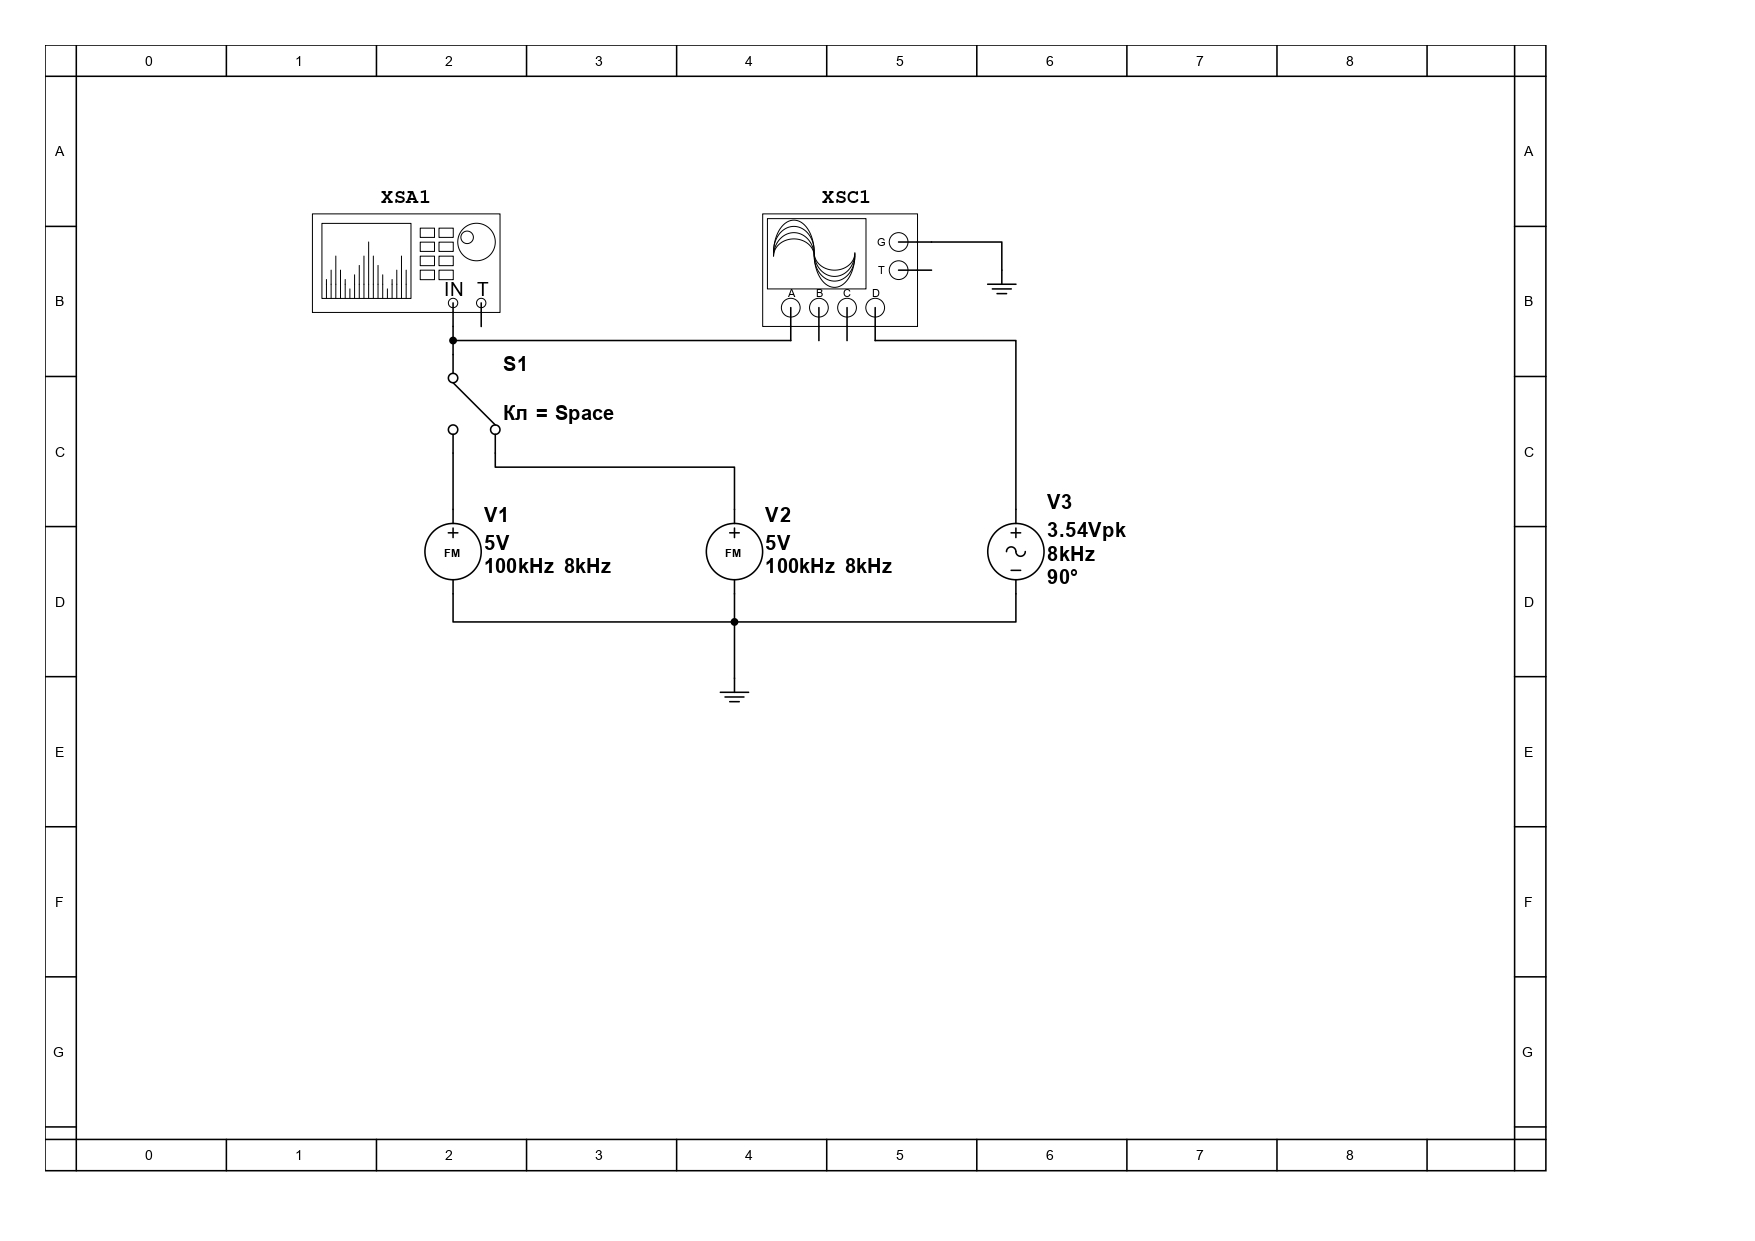
\includegraphics[width=1\linewidth]{img/1/scheme.jpg}
\subsection{<<Схема частотного модулятора и демодулятора>>}
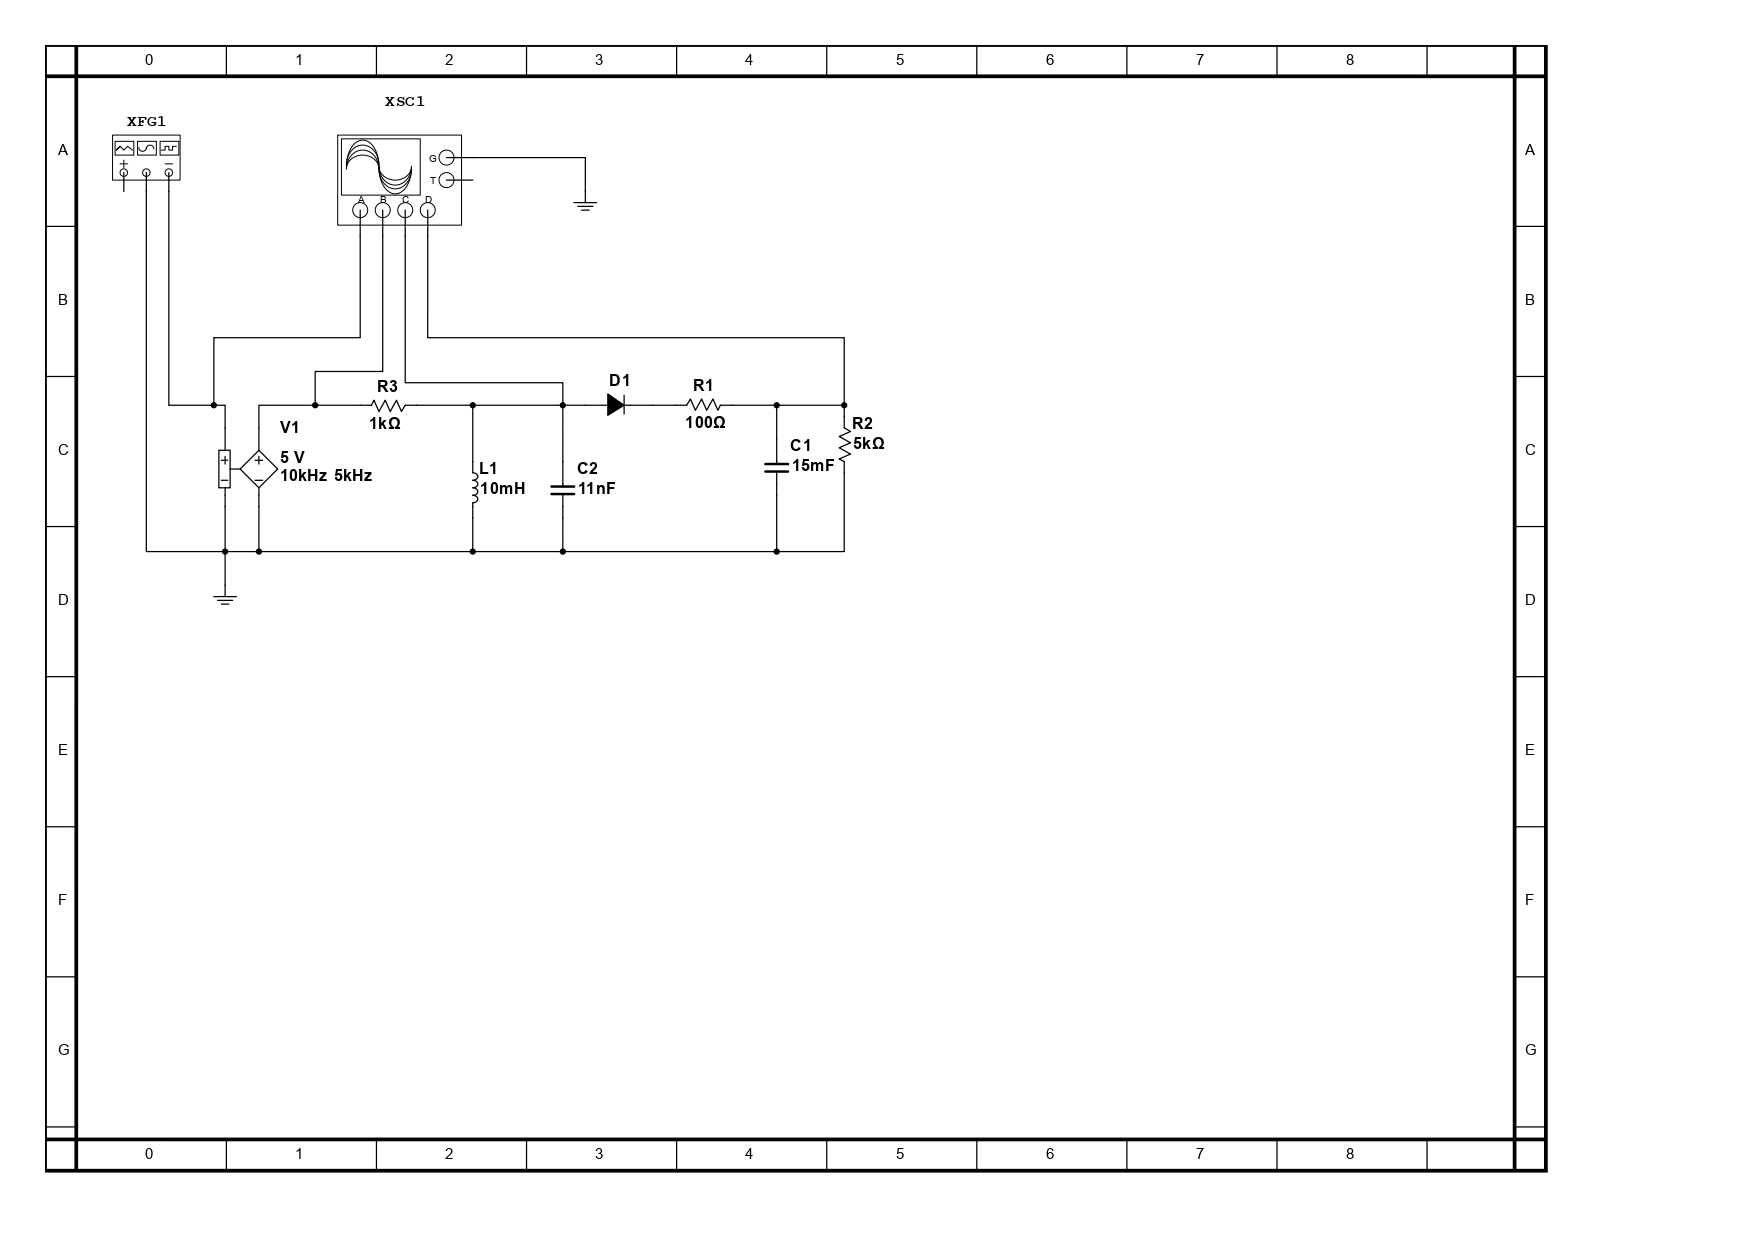
\includegraphics[width=1\linewidth]{img/2/scheme.jpg}
\subsection{<<Схема системы передачи информации с частотной манипуляцией>>}
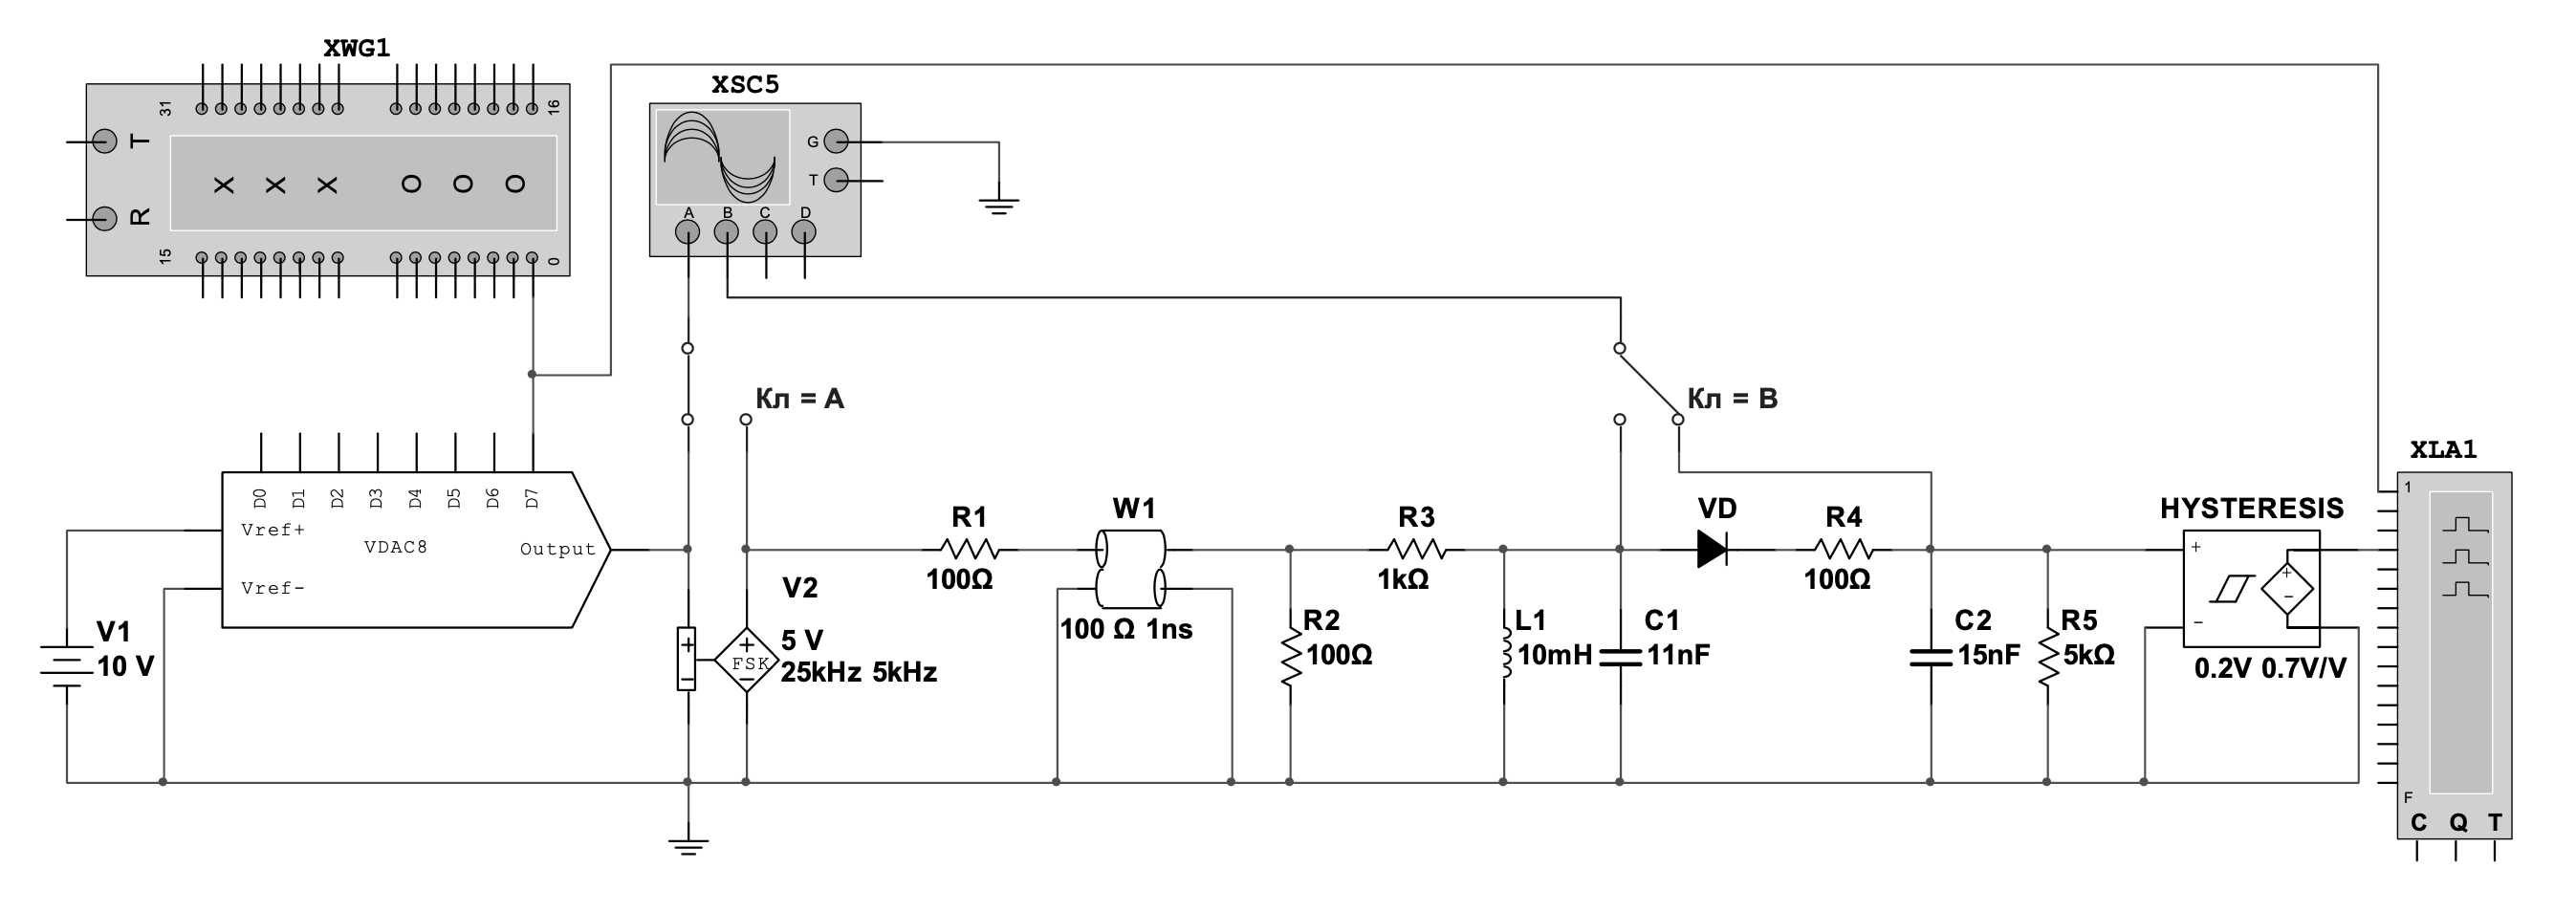
\includegraphics[width=1\linewidth]{img/3/scheme.png}
\section{Результаты расчетов и измерений приборами}
\subsection{<<Схема исследования ЧМ сигналов>>}
\begin{itemize}
\item Ключ открыт:\\
Осциллограмма:\\
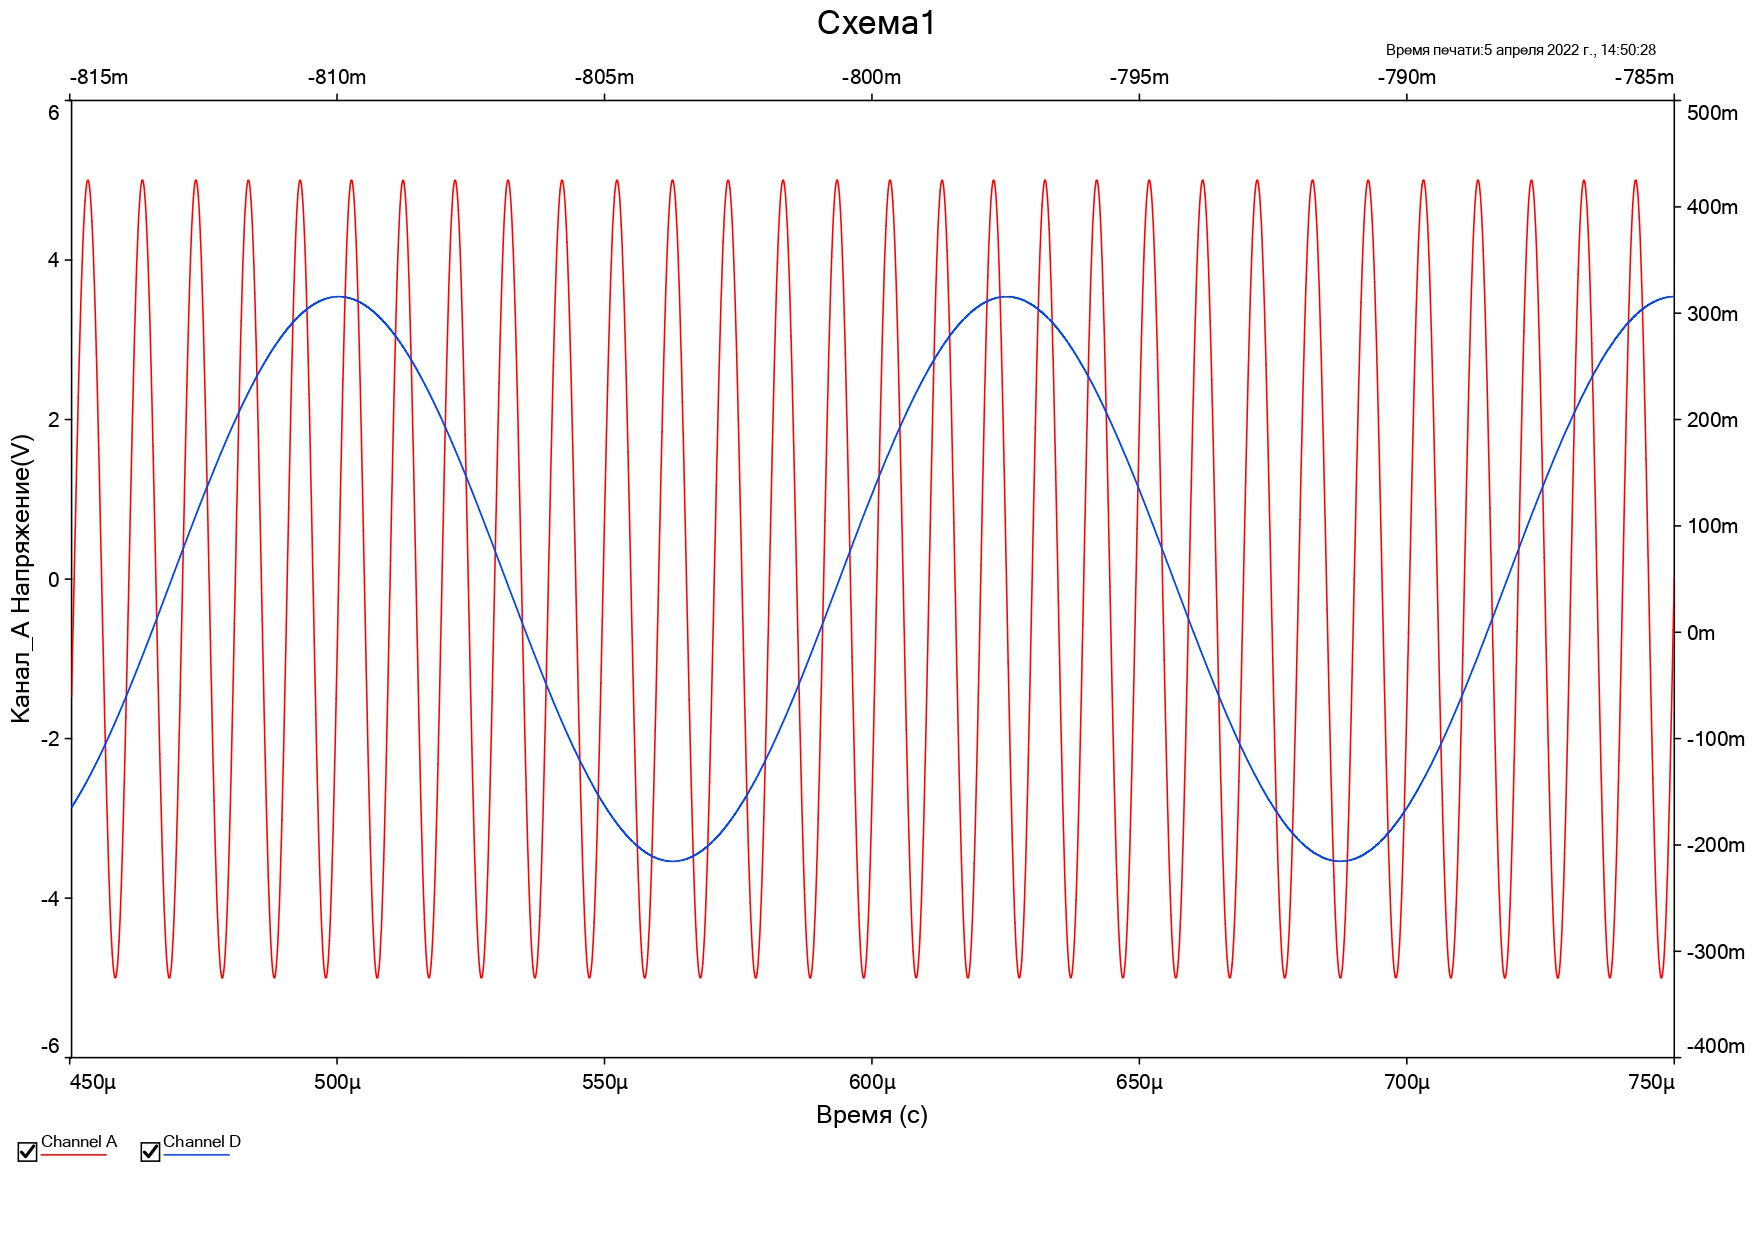
\includegraphics[width=1\linewidth]{img/1/key_open/osc.jpg}
Спектрограмма:\\
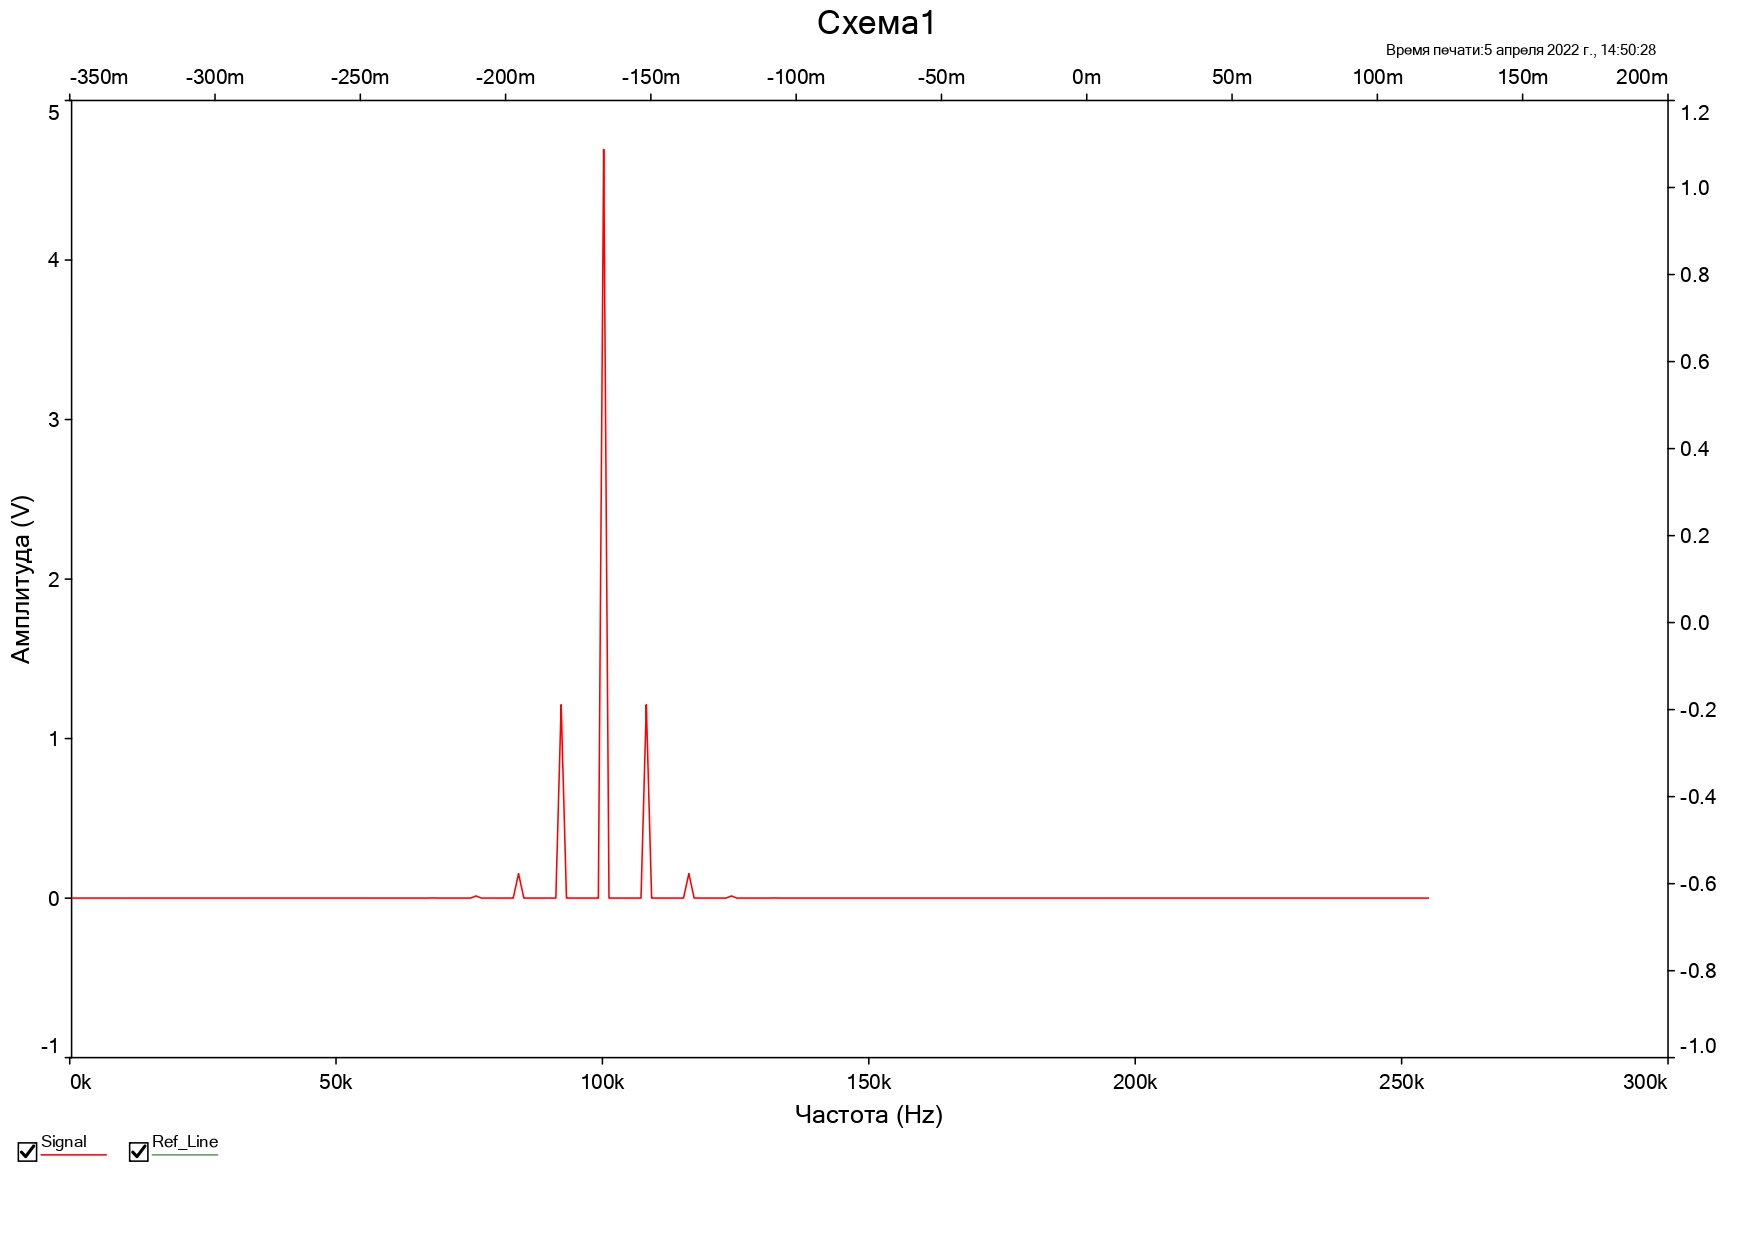
\includegraphics[width=1\linewidth]{img/1/key_open/specter.jpg}
\item Ключ закрыт:\\
Осциллограмма:\\
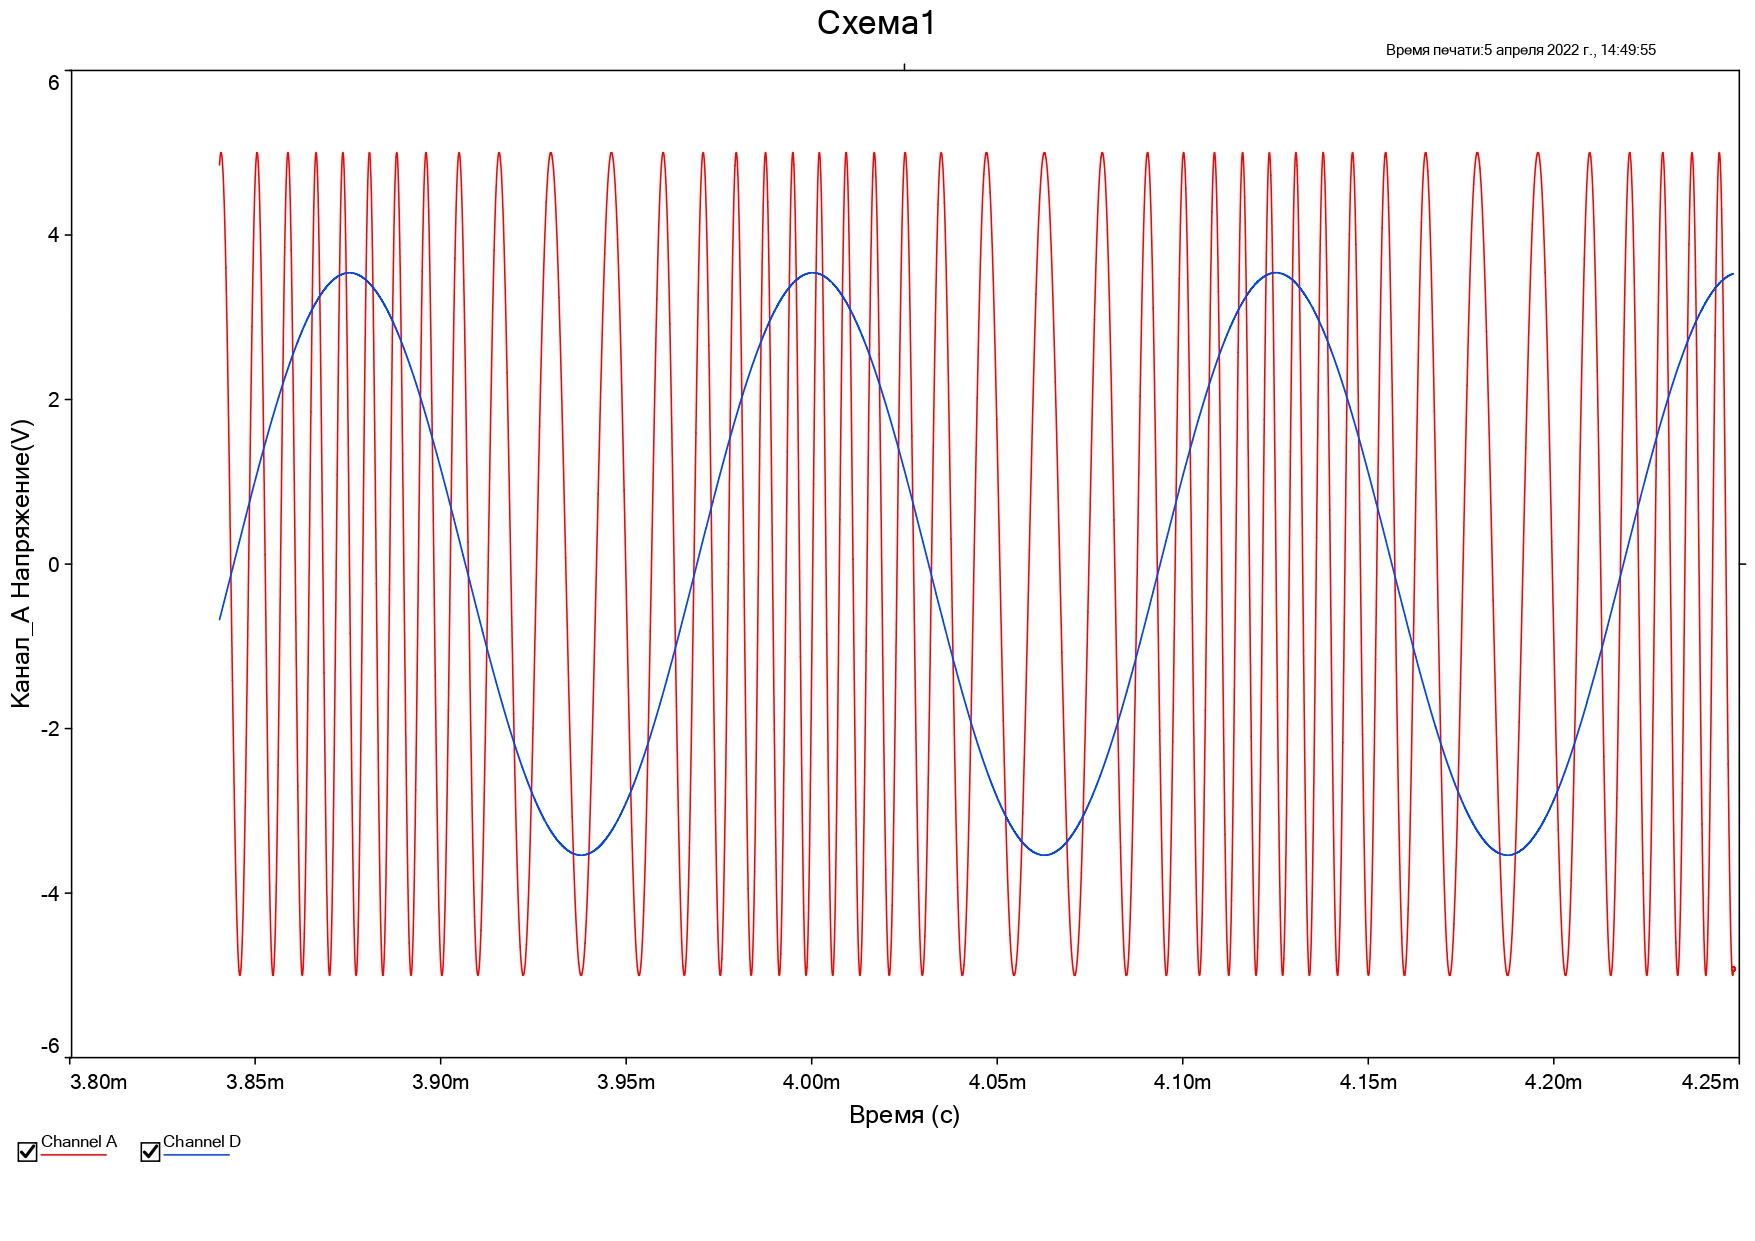
\includegraphics[width=1\linewidth]{img/1/key_closed/osc.jpg}
Спектрограмма:\\
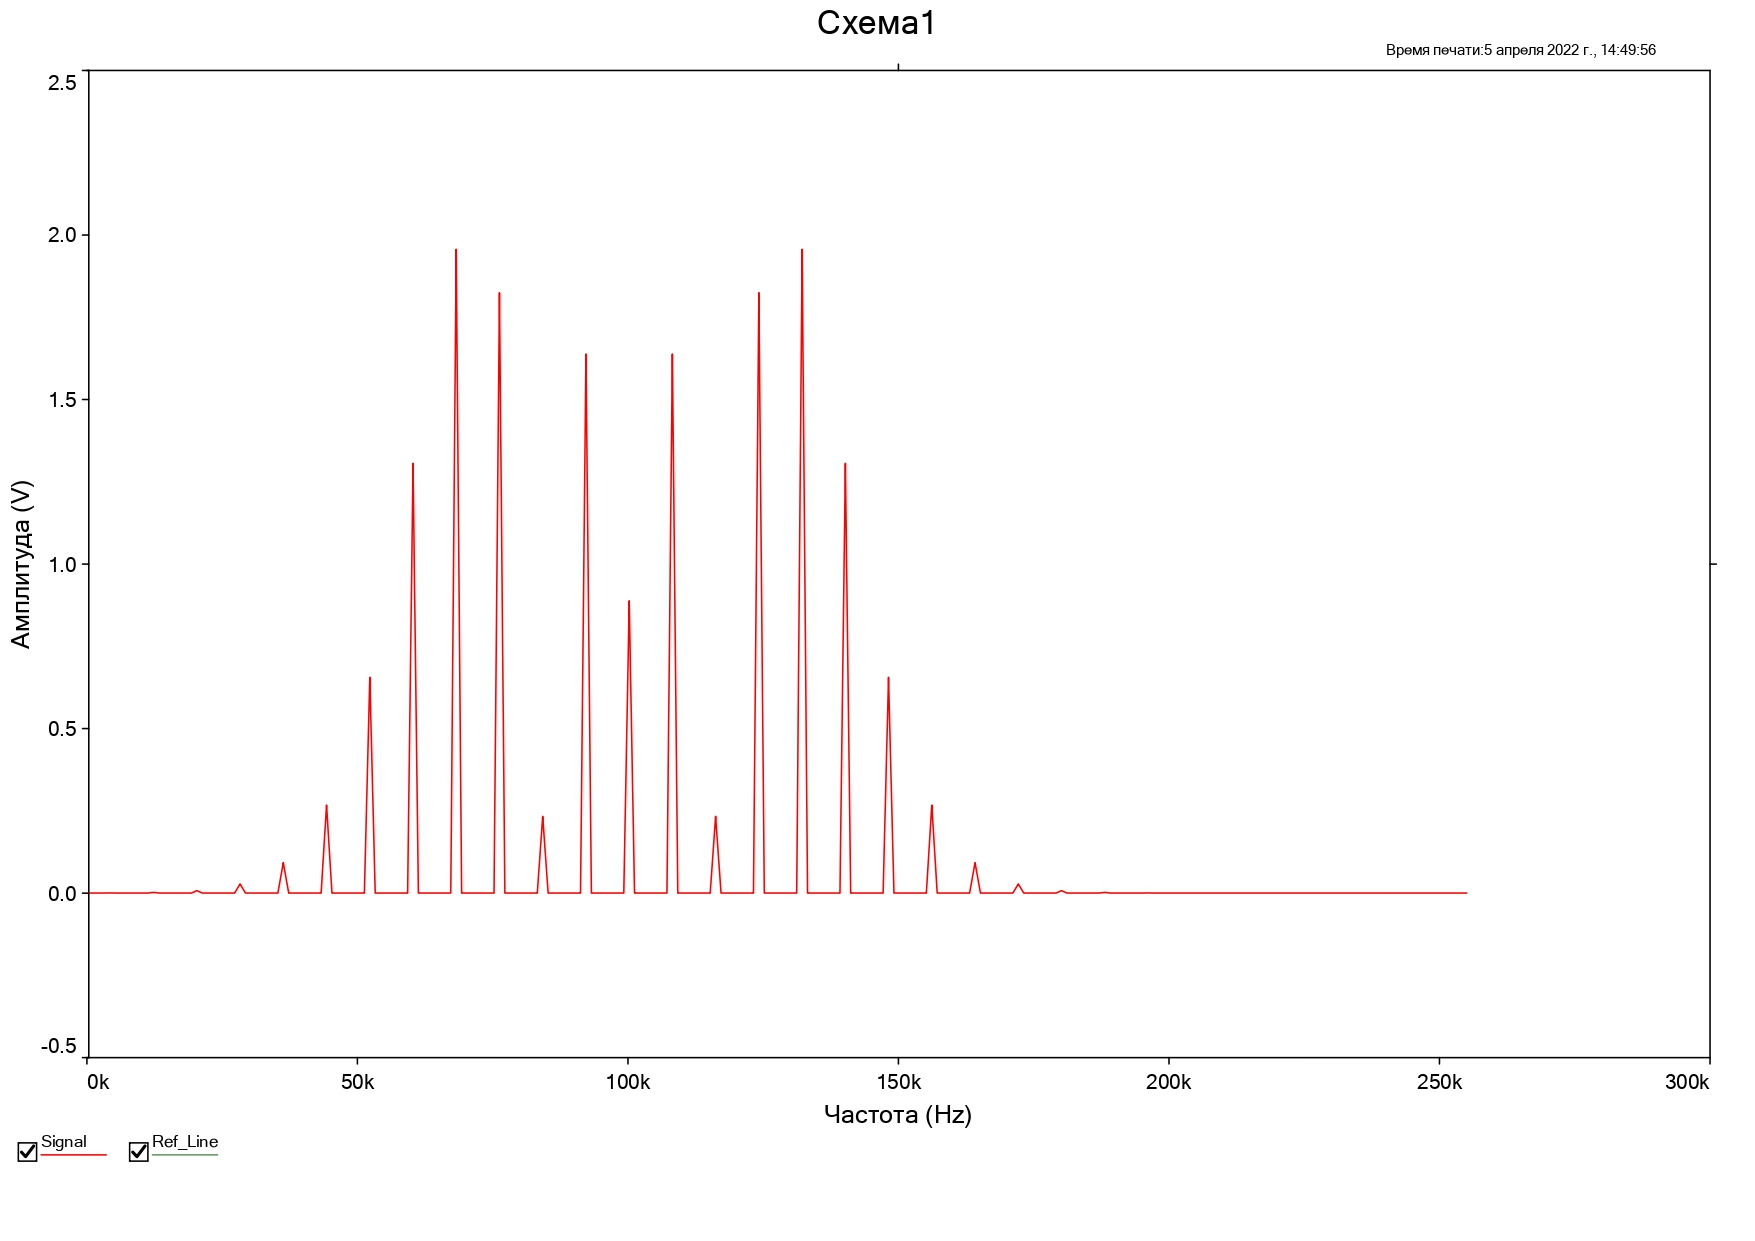
\includegraphics[width=1\linewidth]{img/1/key_closed/specter.jpg}
\end{itemize}
\subsection{<<Схема частотного модулятора и демодулятора>>}
Осциллограмма:\\
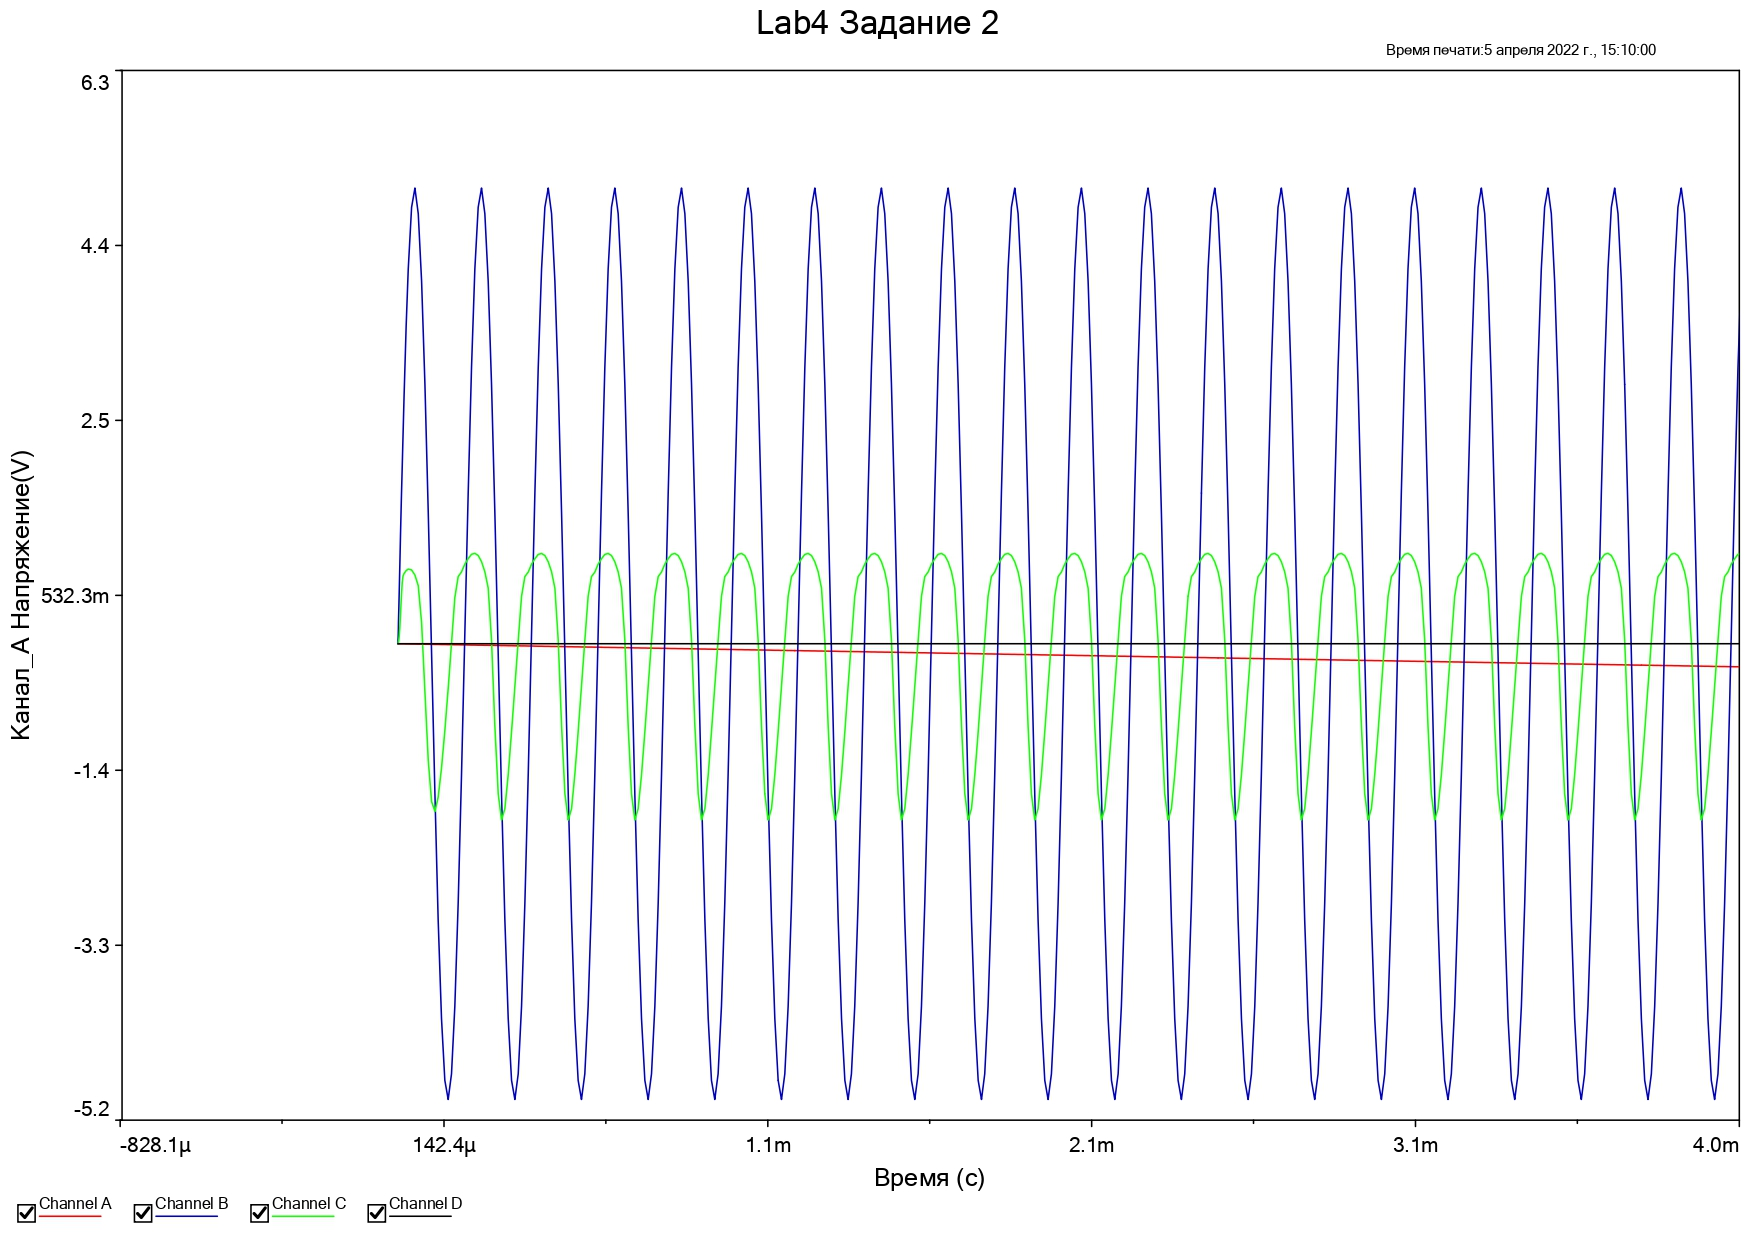
\includegraphics[width=1\linewidth]{img/2/osc2.jpg}
\subsection{<<Схема системы передачи информации с частотной манипуляцией>>}
Осцилограммы:\\
\begin{itemize}
\item Скорость 1 Кбит/c:\\
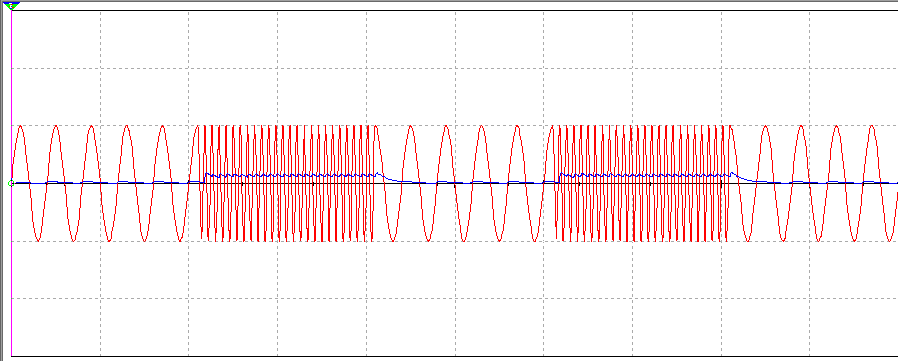
\includegraphics[width=1\linewidth]{img/3/pic3_1.png}
\item Скорость 5 Кбит/c:\\
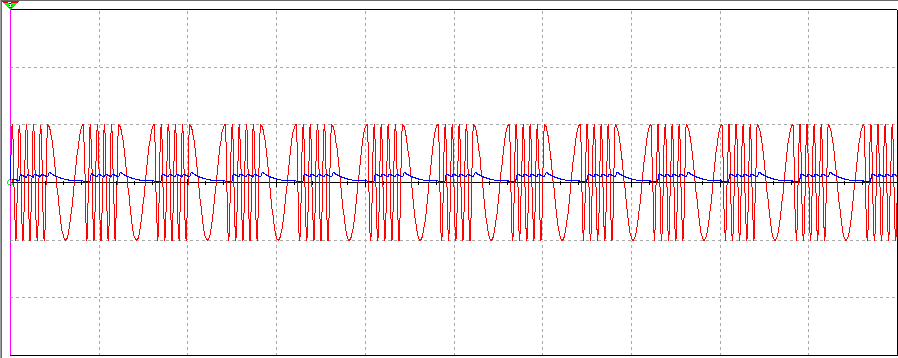
\includegraphics[width=1\linewidth]{img/3/pic3_2.png}
\item Скорость 10 Кбит/c:\\
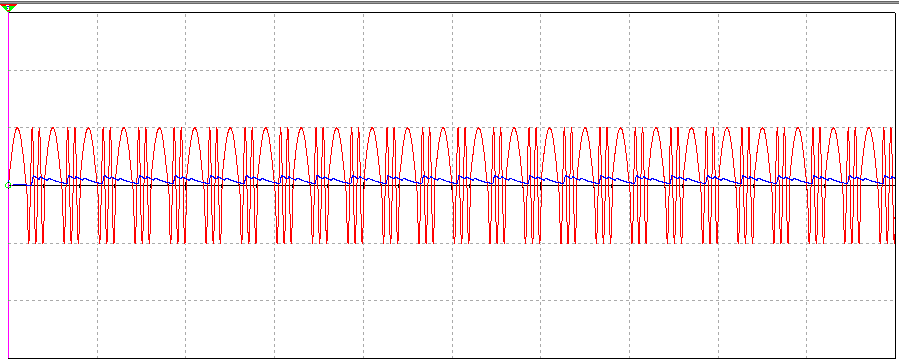
\includegraphics[width=1\linewidth]{img/3/pic3_3.png}
\end{itemize}
\textbf{Вывод:} в ходе выполнения лабораторной работы мы изучили суть передачи бинарных данных по сетям связи, а также принципы работы и построения частотного модулятора и демодулятора.
\end{document}

